 \documentclass[a4paper,12pt]{article}
\usepackage[a4paper,top=1.3cm,bottom=2cm,left=1.5cm,right=1.5cm,marginparwidth=0.75cm]{geometry}
\usepackage{setspace}
\usepackage{cmap}					
\usepackage{mathtext} 				
\usepackage[T2A]{fontenc}			
\usepackage[utf8]{inputenc}			
\usepackage[english,russian]{babel}
\usepackage{multirow}
\usepackage{graphicx}
\usepackage{wrapfig}
\usepackage{tabularx}
\usepackage{float}
\usepackage{longtable}
\usepackage{hyperref}
\hypersetup{colorlinks=true,urlcolor=blue}
\usepackage[rgb]{xcolor}
\usepackage{amsmath,amsfonts,amssymb,amsthm,mathtools} 
\usepackage{icomma} 
\mathtoolsset{showonlyrefs=true}
\usepackage{euscript}
\usepackage{mathrsfs}

\DeclareMathOperator{\sgn}{\mathop{sgn}}
\newcommand*{\hm}[1]{#1\nobreak\discretionary{}
	{\hbox{$\mathsurround=0pt #1$}}{}}
 
 \title{Физический маятник. (1.4.1 В)}
 \author{Павлушкин Вячеслав}
 \date{September 2021}
 
 
 \begin{document}
 	
 	\maketitle
 	
 	\section{Введение}
 	
 	\textbf{Цели работы:} 1) на примере измерения периода свободных колебаний физического
 	маятника познакомиться с систематическими и случайными погрешностями, прямыми и косвенными измерениями; 2) проверить справедливость формулы для периода колебаний физического маятника и определить значение ускорения свободного падения; 3) убедиться в справедливости теоремы Гюйгенса об обратимости
 	точек опоры и центра качания маятника; 4) оценить погрешность прямых и косвенных измерений и конечного результата.\\
 	\textbf{Оборудование:} металлический стержень; опорная призма; торцевые
 	ключи; закреплённая на стене консоль; подставка с острой гранью для определения
 	цента масс маятника; секундомер; линейки металлические длиной 30, 50 и 100 см;
 	штангенциркуль; электронные весы; математический маятник (небольшой груз,
 	подвешенный на нитях).
 	
 	\section{Теоретические сведения}
 	
 	\begin{wrapfigure}{l}{6cm}
 		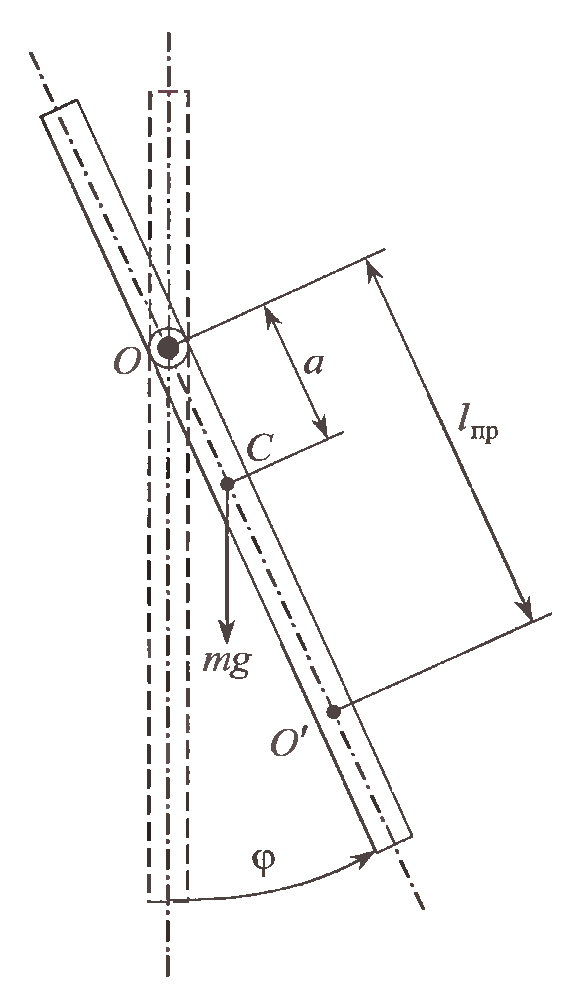
\includegraphics[width=1\linewidth]{ustanovka}
 		\caption{Физический маятник}\label{risunok}
 	\end{wrapfigure}
 	
 	\par В работе изучается динамика движения физического маятника.
 	Физический маятник, используемый в работе, представляет собой однородный стальной стержень массы $m$, длина которого $l$ много больше ее диаметра. На стержне закрепляется опорная призма, острое ребро которой является осью качания маятника.
 	
 	Второй закон Ньютона определяет динамику движения тела точечной массы m. Импульс тела $P=mv$ изменяется во времени $t$ под действием силы $F$:
 	\begin{equation}
 		F = \frac{dP}{dt}
 	\end{equation}
 	Если рассмотреть точечную массу, которая движется по окружности радиуса $r$ с угловой скоростью $\omega$, тогда линейная скорость $v = \omega r$, то формулу для силы можно преобразовать:
 	\begin{equation}
 		Fr = \frac{dP}{dt}r
 	\end{equation}
 	\begin{equation}
 		M=\frac{dP}{dt}r=\frac{dL}{dt}
 	\end{equation}
 	\noindent где $L = J\omega$, и $J = mr^2$. Величину $J$ называют \textit{моментом инерции}.
 	\begin{equation}
 		J = \sum_{i=1} m_i r_i^2
 	\end{equation}
 	\par Посчитаем момент инерции для данного нам стержня, при вращении вокруг препендикулярной стержню оси. Для этого разобьем стержень на отрезки $dr$ и $dm = m\cdot\frac{dr}{l}$ и возьмем интеграл:
 	\begin{equation}
 		J_c = \int_{-\frac{l}{2}}^{\frac{l}{2}}r^2dm = \int_{-\frac{l}{2}}^{\frac{l}{2}}\frac{mr^2}{l}dm = \frac{ml^2}{12} 
 	\end{equation}
 	
 	
 	Призму можно перемещать вдоль стержня, меняя таким образом расстояние $ OC $ от точки опоры маятника до его центра масс. Пусть это расстояние равно $ a $. Тогда по теореме Гюйгенса-Штейнера момент инерции маятника
 	
 	\begin{equation}
 		J=\frac{ml^2}{12}+ma^2,
 	\end{equation}
 	
 	\noindent где $ m $ -- масса маятника.
 	
 	
 	Период колебаний получим через аналогию с пружинным маятником, как известно: \begin{equation}
 		T_\text{п}=2\pi\sqrt{\frac{m}{k}}
 	\end{equation}
 	\noindent В нашем случае, роль массы играет \textit{момент инерции тела $J$}, а \textit{жесткость пружины $k$} - коэффицент пропорциональности $mga$. Таким образом приходим к следующей формуле колебаний произвольного физического маятника:
 	\begin{equation}
 		T=2\pi\sqrt{\frac{J}{mga}}
 	\end{equation}
 	\noindent После подстановки период колебаний, для стержня длиной $l$ подвешенного на расстоянии $a$ от центра, равен:
 	
 	\begin{equation}\label{time_a}
 		T=2\pi\sqrt{\frac{a^2+\frac{l^2}{12}}{ag}}
 	\end{equation}
 	
 	Таким образом, период малых колебаний не зависит ни от начальной фазы, ни от амплитуды колебаний.
 	\medspace
 	
 	Период колебаний математического маятника определяется формулой
 	\begin{equation}
 		T_\text{м}=2\pi\sqrt{\frac{l}{g}},
 	\end{equation}
 	где $ l $ -- длина математического маятника. Поэтому величину
 	\begin{equation}\label{prived}
 		l_\text{пр}=a+\frac{l^2}{12a}
 	\end{equation}
 	называют приведённой длиной математического маятника. Поэтому точку $ O' $ (см. рис. \ref{risunok}), отстоящую от точки опоры на расстояние $ l_\text{пр} $, называют центром качания физического маятника. Точка опоры и центр качания маятника обратимы, т.е. при качании маятника вокруг  точки $ O' $ период будет таким же, как и при качании вокруг точки $ O $.
 	
 	\section {Экспериментальная установка}
 	Тонкий стальной стержень, подвешенный на прикрепленной к стене консоли с помощью небольшой призмы, которая опирается на поверхность консоли острым основанием. Призму можно перемещать вдоль стержня, изменяя положение точки подвеса. Период колебаний измеряется с помощью секундомера, расстояния измеряются линейкой и штангенциркулем. Положение центра масс можно определить с помощью балансирования маятника на вспомогательной подставке.
 	
 	
 	
 	\subsection{Расчет поправок}
 	Если быть честными, то для вычисления периода следует использовать формулу, учитывающую оба тела (и стержень, и призму):
 	\begin{equation}
 		T = 2\pi\sqrt{\frac{J_\text{ст} + J_\text{пр}}{m_\text{ст}ga_\text{ст}-m_\text{пр}ga_\text{пр}}}
 	\end{equation}
 	Однако призма мала по размеру и массе, поэтому поправка на момент инерции призмы в условиях опыта составляет не более 0,1\% $\Rightarrow$ ей можно пренебречь.
 	
 	Сравним теперь моменты сил, действующие на призму и стержень при $a = 10$ см:
 	\begin{equation}
 		\frac{M_\text{пр}}{M_\text{ст}} = \frac{m_\text{пр}ga_\text{пр}}{m_\text{ст}ga_\text{ст}} \approx 10^-2
 	\end{equation}
 	
 	В данном случае поправка достигает 1\% $\Rightarrow$ ей пренебречь нельзя. Учесть влияние призмы можно -- исключив $a_\text{пр}$, изменяя положение центра сиситемы. Пусть $X$ -- расстояние от центра масс системы до точки подвеса, тогда:
 	\begin{equation}
 		X=\frac{m_\text{ст}a_\text{ст}-m_\text{пр}a_\text{пр}}{m_\text{ст} + m_\text{пр}}
 	\end{equation}
 	
 	
 	Исключая из двух уравнений $a_\text{пр}$, получаем:
 	\begin{equation}\label{period}
 		T = 2\pi \sqrt{\frac{\frac{l^2}{12}+a^2}{g\beta X}}
 	\end{equation}	
 	\noindent где $\beta= 1+\frac{m_\text{пр}}{m_\text{ст}}$.
 	\section{Задание}
 	\subsection{Оценка погрешностей измерительных приборов и $g$}
 	\textbf{Секундомер:} $ \sigma_c = 0,01 \text{ с}$\\
 	\textbf{Линейка:} $ \sigma_\text{лин} = 0,05 \text{ см}$\\\\
 	Погрешность $g$ зависит от точности измерения длин и периода колебаний. Длины измеряли линейкой. Наименьшее измеренное расстояние 15 см, а наибольшее 100 см. Абсолютная погрешность линейки: $\sigma_\text{лин} = 0,05 \text{ см}$. Тогда относительная погрешность длин составляет порядка $\varepsilon_\text{max}\approx0,3\%$  ($\frac{0,05см}{15см}\times100\% = 0,3\%$).\\\\
 	\textbf{Вывод:} используемые в работе инструменты позволяют вести измерения длин с точностью вплоть до 0,1\%. Для получения конечного результата с данной точностью период колебаний следует измерять с той же относительной погрешностью: не хуже, чем $\varepsilon_\text{max}\approx0,3\%$.
 	\subsection{Длина стержня и множитель $\beta$}
 	
 	Длина стержня $l = \left(  100,1 \pm 0,05\right)$ см, масса стержня $m =\left(  868,9 \pm 0,1\right)$ г, масса призмы $m_\text{пр}=\left( 73,9 \pm 0,1\right)$ г. Формула для множителя $\beta$:
 	\begin{equation}
 		\beta=1+\frac{m_\text{пр}}{m}
 	\end{equation}
 	
 	\noindent Рассчитаем множитель используя снятые массы: $\beta = 1+\frac{73,9}{868,9}\approx1,08505$. Погрешность $\beta$ $\sigma_\text{$\beta$}$ будет рассчитывается по формуле:
 	\begin{equation}
 		\sigma_\text{$\beta$}=\beta\sqrt{\left(\frac{\sigma_\text{пр}}{m_\text{пр}}\right)^2+\left(\frac{\sigma}{m}\right)^2}
 	\end{equation}
 	\begin{equation}
 		\sigma_\text{$\beta$}=1,08505\sqrt{\left(\frac{0,1}{73,9}\right)^2+\left(\frac{0,1}{868,9}\right)^2}\approx0,00147
 	\end{equation}
 	\par Получаем, что $\beta = \left( 1,08505 \pm 0,00147\right)$ с учетом погрешности. В соответствии с правилами округления получаем, что $\beta$ следует округлять до четырех знаков после запятой: $\beta = \left( 1,0851 \pm 0,0015\right)$.
 	
 	\subsection{Центр масс стержня и конструкции}
 	Центр масс стержня расположен на расстоянии $b = (50, 10 \pm 0,05) \text{ см}$ от одного из его концов. Острие призмы расположено на расстоянии $a = (24,90 \pm 0,05) \text{ см}$. 
 	Сбалансировав маятник \emph{с призмой} на острие вспомогательной установки, измерим положение центра масс конструкции $x_\text{ц} = 23,0\text{ см}$. Определение точного положения центра масс усложняется тем, что достичь точного равновесия конструкции на установке почти невозможно, поэтому погрешность измерения увеличится: $x_\text{ц} = (23,0 \pm 0,1)\text{ см}$.
 	
 	\subsection{Предварительный опыт}
 	Установим маятник на консоли и отклоним его на малый угол $\varphi_0 \approx 5^\circ$. Измерим время $n = 10$ полных колебаний и вычислим период колебаний $T = t/n$. Результаты 10 измерений приведем в таблице \ref{tab1}.
 	\begin{table}[H]
 		\begin{center}
 			\begin{tabular}{|c|c|c|c|c|c|c|c|c|c|c|c|}
 				\hline
 				№ & 1 & 2 & 3 & 4 & 5 & 6 & 7 & 8 & 9 & 10 & ср. \\
 				\hline
 				$t$, c & 15,37 & 15,42 & 15,37 & 15,24 & 15,35 & 15,31 & 15,43 & 15,28 & 15,39 & 15,36 & 15,35\\ 
 				\hline
 				$T$, с & 1,537 & 1,542 & 1,537 & 1,524 & 1,535 & 1,531 & 1,543 & 1,528 & 1,539 & 1,536 & 1,535\\ 
 				\hline
 				$\Delta t$, c& 0,02 & 0,07 & 0,02 & 0,11 & 0,00 & 0,04 & 0,08 & 0,07 & 0,04 & 0,01 & \\
 				\hline
 			\end{tabular}
 		\end{center}
 		\caption{Результаты измерения периода колебаний}
 		\label{tab1}
 	\end{table}
 	
 	Предварительное значение ускорения свободного падения посчитаем по формуле
 	\begin{equation}\label{golos}
 		g = \frac{4\pi^2 (\frac{l^2}{12} + a^2)}{T^2 \beta x_\text{ц}}
 	\end{equation}
 	\par Полученное значение равно $g = 9,76$ м/с$^2$. Отличие от табличного значения $g = 9,81$ м/с$^2$ составляет 
 	\begin{equation}
 		\alpha = \frac{9,81 - 9,76}{9,81}\times100\% = 0,51\%
 	\end{equation}
 	\par Случайная погрешность измерения времени составляет
 	\begin{equation}
 		I_\text{ц}.
 	\end{equation}
 	\par Полная погрешность измерения времени составляет
 	\begin{equation}
 		\sigma_\text{t} = \sqrt{\sigma_\text{случ}^2+\sigma_\text{с}^2} = 0,061\text{ c}.
 	\end{equation}
 	\par Следовательно, с учетом погрешности период колебаний равен $T = 1,535 \pm 0,007$ с.
 	
 	\subsection{Оценка количества колебаний}
 	\par Оценим количество колебаний маятника, по которому следует измерять его период. Период составляет $T \approx 1,5\text{ c}$. Поскольку $T = t/n$, погрешность периода равна $\sigma_\text{T} = \sigma_\text{t}/n$. Относительная погрешность $\varepsilon_\text{T}/T = \varepsilon_\text{t}/nT$. При требуемой погрешности $\varepsilon = 0,3\%$ получим $n \approx 10-15$.
 	
 	\subsection{Измерение периода колебаний для различных значений $\text{a}$}
 	
 	Изменяем положение призмы, каждый раз измеряя ее положение $a$ относительно центра, положение центра масс системы $x_\text{ц}$ и время $n$ полных колебаний. Результаты приведены в таблице \ref{tab2}.
 	
 	\begin{table}[H]
 		\begin{center}
 			\begin{tabular}{|c|c|c|c|c|c|c|c|c|c|c|}
 				\hline
 				№ & 1 & 2 & 3 & 4 & 5 & 6 & 7 & 8 & 9\\
 				\hline
 				$\text{a}$, см & 41,0 & 37,0 & 33,0 & 29,0 & 24,9 & 20,0 & 15,0 & 10,0 & 5,0\\
 				\hline
 				$x_\text{ц}$, см & 37,9 & 34,0 & 30,2 & 26,7 & 23,0 & 18,4 & 13,6 & 9,2 & 4,4\\
 				\hline
 				$n$ & 10 & 10 & 10 & 10 & 10 & 10 & 10 & 10 & 10\\
 				\hline
 				$t_1$, с & 15,70 & 15,61 & 15,34 & 15,28 & 15,37 & 15,91 & 17,02 & 19,48 & 26,64\\
 				\hline
 				$t_2$, с & 15,71 & 15,56 & 15,29 & 15,14 & 15,42 & 15,92 & 16,86 & 19,45 & 26,62\\
 				\hline
 				$t_3$, с & 15,77 & 15,54 & 15,29 & 15,24 & 15,37 & 15,71 & 16,88 & 19,52 & 26,72\\
 				\hline
 				$t_4$, с & 15,67 & 15,57 & 15,27 & 15,31 & 15,24 & 15,82 & 16,90 & 19,48 & 26,88\\
 				\hline
 				$t_5$, с & 15,81 & 15,52 & 15,29 & 15,31 & 15,35 & 15,89 & 16,90 & 19,43 & 26,66\\
 				\hline
 				$t_6$, с & 15,86 & 15,47 & 15,26 & 15,28 & 15,31 & 15,73 & 16,90 & 19,58 & 26,67\\
 				\hline
 				$t_7$, с & 15,81 & 15,62 & 15,23 & 15,30 & 15,43 & 15,69 & 16,92 & 19,53 & 26,75\\
 				\hline
 				$t_8$, с & 15,60 & 15,42 & 15,38 & 15,26 & 15,28 & 15,80 & 16,99 & 19,54 & 26,74\\
 				\hline
 				$t_9$, с & 15,83 & 15,55 & 15,38 & 15,38 & 15,39 & 15,94 & 16,92 & 19,33 & 26,87\\
 				\hline
 				$t_10$, с & 15,75 & 15,46 & 15,34 & 15,36 & 15,36 & 15,93 & 16,90 & 19,51 & 26,75\\
 				\hline
 				$t_\text{ср}$, с & 15,75 & 15,53 & 15,31 & 15,29 & 15,35 & 15,83 & 16,92 & 19,49 & 26,73\\
 				\hline
 				$T_\text{ср}$, с & 1,575 & 1,553 & 1,531 & 1,529 & 1,535 & 1,583 & 1,692 & 1,949 & 2,673\\
 				\hline
 				$g, \text{м/с}^2$ & 9,74 & 9,78 & 9,89 & 9,77 & 9,77 & 9,74 & 9,91 & 9,74 & 9,95\\
 				\hline
 				$\Delta g, \text{м/с}^2$ & 0,07 & 0,03 & 0,08 & 0,04 & 0,04 & 0,07 & 0,10 & 0,07 & 0,14\\
 				\hline
 			\end{tabular}
 		\end{center}
 		\caption{Результаты измерения периода колебаний для различных $\text{a}$}
 		\label{tab2}
 	\end{table}        
 	
 	\subsection{Определение приведенной длины маятника}
 	Для $a = 15,0$ см:
 	\begin{equation}
 		l_\text{прив} = a + \frac{l^2}{12a} = 15 + \frac{100,1^2}{12\times 15} \approx 70,7 \text{ см.}
 	\end{equation}
 	Установим соответствующую длину математического маятника и проведем серию измерений времени $n = 10$ колебаний. Результаты приведены в таблице \ref{tab3}:
 	\begin{table}[H]
 		\begin{center}
 			\begin{tabular}{|c|c|c|c|c|c|c|c|c|c|c|c|}
 				\hline
 				№ & 1 & 2 & 3 & 4 & 5 & 6 & 7 & 8 & 9 & 10 & ср.\\
 				\hline
 				$t^\text{'}$, с & 16,90 & 16,98 & 16,95 & 17,02 & 16,87 & 16,95 & 16,90 & 16,79 & 16,83 & 16,97 & 16,92\\
 				\hline
 				$T^\text{'}$, с & 1,690 & 1,698 & 1,695 & 1,702 & 1,687 & 1,695 & 1,690 & 1,679 & 1,683 & 1,697 & 1,692\\
 				\hline
 				$\Delta t^\text{'}$, с & 0,02 & 0,06 & 0,03 & 0,10 & 0,05 & 0,03 & 0,02 & 0,03 & 0,09 & 0,05 & ---\\
 				\hline
 			\end{tabular}
 		\end{center}
 		\caption{Результаты измерения периода колебаний математического маятника}
 		\label{tab3}
 	\end{table}
 	
 	Период колебаний физического маятника при $a$ = 15 см -- $T$ = 1,692 с $\Rightarrow$ физический маятник длиной $l$, подвешенный 
 	в точке $a$, имеет тот же период малых колебаний, что и математический 
 	маятник длиной $l_\text{пр}$.
 	
 	\subsection{Центр качания}
 	Для $a$ = 29,0 см $l_\text{пр}$ = 57,8 см. Закрепим призму так, чтобы ее острие находилось в центре качания маятника, т.е. на расстоянии $l_\text{пр}$ от предыджущего ее положения. Проведем серию измерений времени $n = 10$ полных колебаний. Результаты приведены в таблице \ref{tab4}.
 	
 	\begin{table}[H]
 		\begin{center}
 			\begin{tabular}{|c|c|c|c|c|c|c|}
 				\hline
 				№ & 1 & 2 & 3 & 4 & 5 & ср.\\
 				\hline
 				$T^\text{}$, с & 15,18 & 15,25 & 15,20 & 15,25 & 15,38 & 15,25\\
 				\hline
 				$t^\text{}$, с & 1,518 & 1,525 & 1,520 & 1,525 & 1,538 & 1,525\\
 				\hline
 			\end{tabular}
 		\end{center}
 		\caption{Измерение времени колебаний математического маятника}
 		\label{tab4}
 	\end{table}
 	
 	\section{Обработка результатов измерений}
 	\subsection{Усредненное значение $g$}
 	Усредним значение $g = 9,81 \text{м/с}^2$. 
 	
 	По формуле \eqref{golos} Найдем систематическую погрешность $g$:
 	\begin{equation}
 		\sigma_g^\text{сист} = g\cdot \sqrt{\left(\frac{\sigma_{\frac{l^2}{12}+a^2}}{\frac{l^2}{12}+a^2}\right)^2+\left(\frac{\sigma_{T^2 \beta X}}{T^2\beta X}\right)^2}
 	\end{equation}
 	\begin{equation}
 		\sigma_{\frac{l^2}{12}+a^2} = \sqrt{\left(\sigma_{l^2}^2+\sigma_{a^2}^2 \right)}
 	\end{equation}
	\begin{equation}
 			\sigma_g^\text{сист} =  g\cdot\sqrt{\frac{\left(\frac{2\sigma_l}{l} \right)^2 + \left(\frac{2\sigma_a}{a}\right)^2}{\left(\frac{l^2}{12}+a^2 \right)^2} + \left(\frac{2\sigma_T}{T}\right)^2+\left(\frac{\sigma_{\beta}}{\beta} \right)^2 + \left(\frac{\sigma_{X}}{X} \right)^2}		
 	\end{equation}
 	
 	
 	\begin{equation}
 		\sigma_g^\text{сист} \approx 0,104 \frac{\text{м}}{c^2}
 	\end{equation}
 	
 	
 	Полную погрешность $g$ получим из $\sigma_g^\text{случ}$ и $\sigma_g^\text{сист}$:
 	\begin{equation}
 		\sigma_g^\text{полн} = \sqrt{(\sigma_g^\text{сист})^2+(\sigma_g^\text{случ})^2}\approx 0,133\frac{\text{м}}{c^2}	\end{equation}	
 	где $\sigma_g^\text{случ} = 0,083 \frac{\text{м}}{c^2}   $.
 	
 	Тогда получаем: $g=\left( 9,81\pm 0,13\right) \frac{\text{м}}{c^2}$.
 	
 	\subsection{График $T(a)$}
 	\begin{figure}[h!]
 		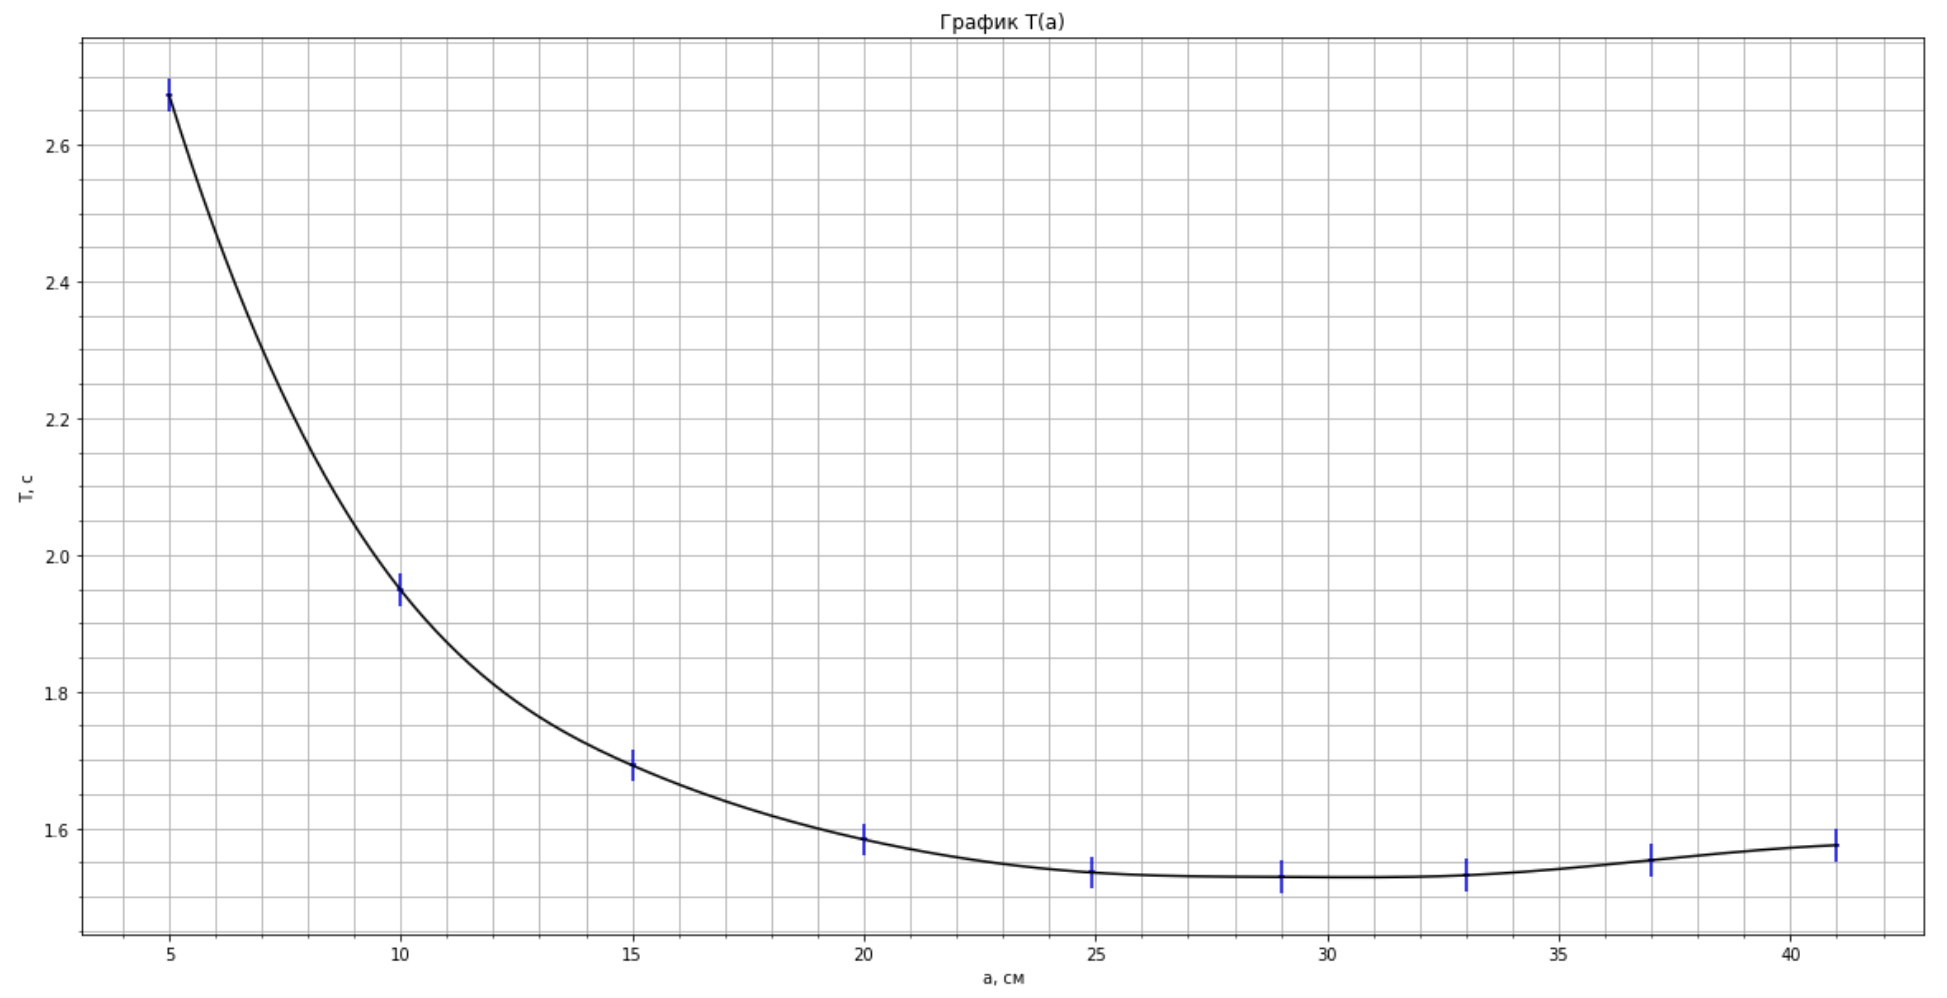
\includegraphics[scale=0.53]{graph}
 		\caption{Зависимость $ T $ от $ a $}
 		\label{graph}
 	\end{figure}
 	
 	
 	Минимум графика (Pисунок \ref{graph}) находится на $a_\text{min} \approx 29$ см, что сходится с рассчетом минимума по формуле \eqref{time_a}: $a_\text{формулы}\approx 28,8$ см
 	\subsection{График зависимости $ T^2 x_\text{ц}\beta $ от $ a^2 $ }
 	Используя формулу для периода физического маятника \eqref{period} получаем следующее соотношение:
 	
 	\begin{equation}
 		T^2x_\text{ц}\beta=\frac{4\pi^2}{g}a^2+\frac{\pi^2l^2}{3g}.
 	\end{equation}
 	Отсюда можно сделать вывод о том, что $ T^2x_\text{ц}\beta $ линейно зависит от $ a^2 $, поэтому это зависимость можно представить в виде
 	
 	\begin{equation}
 		T^2x_\text{ц}\beta=ka^2+b,
 	\end{equation}
 	где
 	\begin{equation}\label{koef}
 		k=\frac{4\pi^2}{g}  \text{ и }  b = \frac{\pi^2l^2}{3g}.
 	\end{equation}
 	
 	
 	График зависимости $ T^2x_\text{ц}\beta $ от $ a^2 $ представлен на рисунке \ref*{graph_file}.
 	
 	\begin{figure}[h!]
 		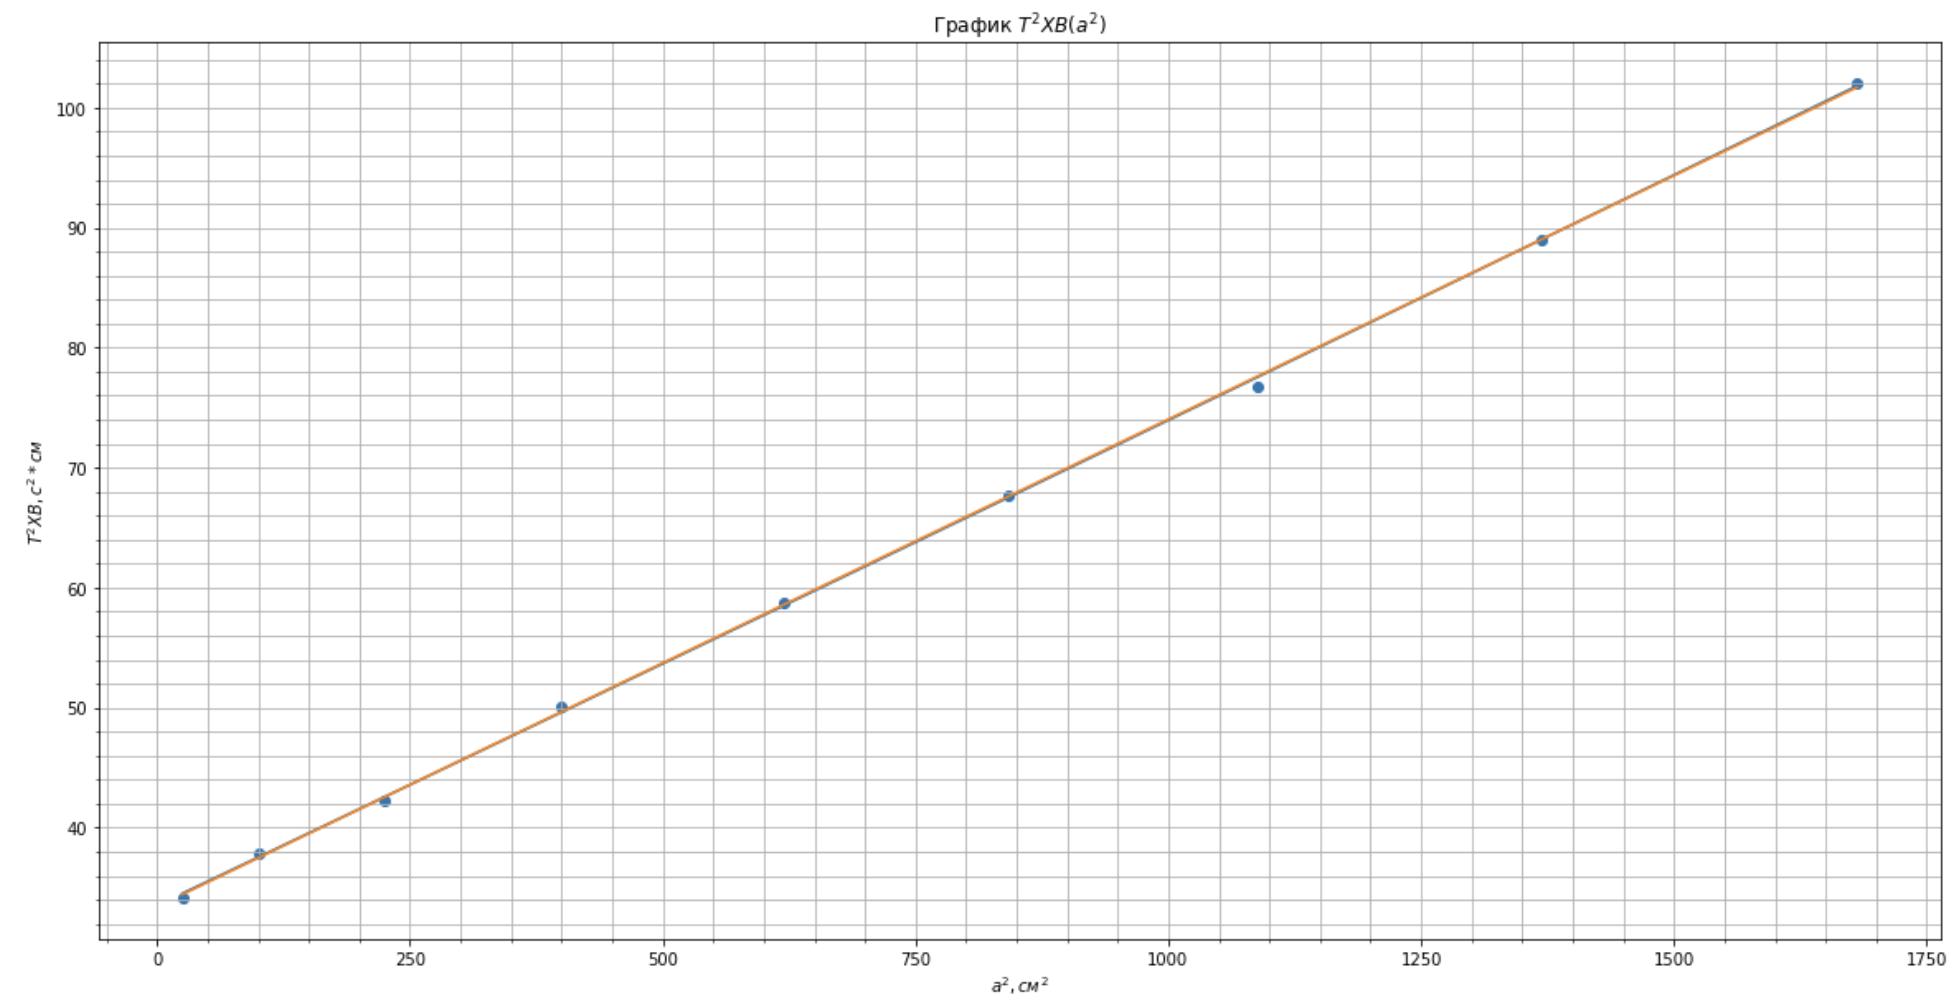
\includegraphics[scale=0.53]{graph_file}
 		\caption{Зависимость $ T^2X\beta $ от $ a^2 $}
 		\label{graph_file}
 	\end{figure}
 	\par
 	Погрешность расчёта $ a^2 $ найдём по следующей формуле:
 	
 	\begin{equation}
 		\varepsilon_{a^2}=2\varepsilon_a=2\frac{\sigma_a}{a}
 	\end{equation}
 	где $ \sigma_a = 0,1$ см.
 	
 	Погрешность вычисления $ T^2x_\text{ц}\beta $ можно найти по формуле:
 	
 	\begin{equation}
 		\varepsilon_{T^2x_\text{ц}\beta} = \sqrt{\left( 2\cdot\frac{\sigma_T}{T} \right)^2 + \left(  \frac{\sigma_X}{X} \right)^2 + \left(\frac{\sigma_{\beta}}{\beta}\right)^2} \approx 0,01  ,
 	\end{equation}
 	
 	Для вычисления коэффициентов $ k $ и $ b $ из \eqref{koef} воспользуемся методом наименьших квадратов:
 	
 	\begin{equation}
 		k=\frac{\langle xy\rangle-\langle x\rangle \langle y\rangle}{\langle x^2\rangle - \langle x\rangle^2}\approx 0,0406\text{ }\frac{\text{с}^2}{\text{см}},
 	\end{equation}
 	
 	\begin{equation}
 		b=\langle y \rangle -k\langle x \rangle\approx 33,54\text{ }\text{см}\cdot\text{с}^2,
 	\end{equation}
 	где $ x=a^2 $, $ y=T^2x_\text{ц}\beta $.
 	
 	Случайные погрешности вычисления $ k $ и $ b $ можно найти по следующим формулам:
 	
 	\begin{equation}
 		\sigma_k^\text{сл}=\frac{1}{\sqrt{N}}\sqrt{\frac{\langle y^2 \rangle - \langle y \rangle^2}{\langle x^2 \rangle - \langle x \rangle^2} - k^2  } \approx 2,08\cdot10^{-4} \text{ }\frac{\text{с}^2}{\text{см}},
 	\end{equation}
 	
 	\begin{equation}
 		\sigma_b^\text{сл}= \sigma_k^\text{сл} \sqrt{\langle x^2 \rangle - \langle x \rangle^2} \approx 0,11 \text{ }\text{см}\cdot\text{с}^2.
 	\end{equation}
 	
 	Систематическая погрешность вычисления коэффициентов определяется следующим соотношением:
 	
 	\begin{equation}
 		\sigma^\text{сист}_k = k\sqrt{\left( \varepsilon_{T^2X\beta} \right)^2 + \left( \varepsilon_{a^2} \right)^2 } \approx 4,5\cdot10^{-4} \text{ }\frac{\text{с}^2}{\text{см}},
 	\end{equation}
 	
 	\begin{equation}
 		\sigma^\text{сист}_b = b\sqrt{\left( \varepsilon_{T^2X\beta} \right)^2 + \left( \varepsilon_{a^2} \right)^2 } \approx  0,37 \text{ }\text{см}\cdot\text{с}^2.
 	\end{equation}
 	
 	Тогда полную погрешность вычисления коэффициентов подсчитываем по следующей формуле:
 	
 	\begin{equation}
 		\sigma_k = \sqrt{\left( \sigma_k^\text{сл} \right)^2 + \left( \sigma_k^\text{сист} \right)^2 } \approx 4,96\cdot 10^{-4} \text{ }\frac{\text{с}^2}{\text{см}},
 	\end{equation}
 	
 	\begin{equation}
 		\sigma_b = \sqrt{\left( \sigma_b^\text{сл} \right)^2 + \left( \sigma_b^\text{сист} \right)^2 } \approx 0,39 \text{ }\text{см}\cdot\text{с}^2.
 	\end{equation}
 	
 	Таким образом, получаем:
 	\begin{itemize}
 		\item $ k = \left( 0,0406\pm 4,96\cdot10^{-4}\right)  \text{ }\frac{\text{с}^2}{\text{см}} $, $ \varepsilon_k = 1,22 \% $
 		\item $ b = \left( 33,54\pm 0,39 \right)  \text{ }\text{см}\cdot\text{с}^2 $, $ \varepsilon_b = 1,16 \% $
 	\end{itemize}
 	
 	Учитывая формулу \eqref{koef}, вычисляем $ g $ через угол наклона прямой:
 	
 	\begin{equation}
 		g_k = \frac{4\pi^2}{k} \approx 9,723  \text{ }\frac{\text{м}}{\text{с}^2},
 	\end{equation}
 	
 	\begin{equation}
 		\sigma_{gk} = g\cdot\varepsilon_k \approx 0,088 \text{ }\frac{\text{м}}{\text{с}^2},
 	\end{equation}
 	
 	
 	
 	Учитывая формулу \eqref{koef}, вычисляем $ g $ через пересечение с осью "y":
 	
 	\begin{equation}
 		g_b = \frac{\pi^2l^2}{3b} \approx 9,809  \text{ }\frac{\text{м}}{\text{с}^2},
 	\end{equation}
 	
 	\begin{equation}
 		\sigma_{gb} = g\cdot\varepsilon_b \approx 0,114 \text{ }\frac{\text{м}}{\text{с}^2},
 	\end{equation}
 	
 	
 	
 	В итоге имеем следующие результаты:
 	
 	\begin{itemize}
 		
 		\item \underline{$ g_k = \left( 9,723\pm 0,088\right) \frac{\text{м}}{\text{с}^2} $, $ \varepsilon_{gk} = 1,22\% $}
 		
 		\item \underline{$ g_b = \left( 9,809\pm 0,114\right) \frac{\text{м}}{\text{с}^2} $, $ \varepsilon_{gb} = 1,16\% $}
 		
 		
 		
 	\end{itemize}
 	
 	
 	Исходя из полученных данных, пожно сказать, что предпочтительнее использовать второй метод определения $g$, а именно нахождение линейной зависимости, определение ее коэффицентов методом наименьших квадратов. При такой обработке данных влияние случайной погрешности будет наименьшим, в отличие от нахождения $g$ по среднему периоду и усреднение $g$.
 	
 	
 	\section{Вывод}
 	Проделанный опыт подтверждает теорию для периода колебаний физического маятника и теорию о приведенной длине физического маятника. Также, мы убедились в справедливости теоремы Гюйгенса об обратимости точек опоры и центра качания маятника.
 	
 	В ходе работы мы получили следующие величины:
 	\begin{itemize}
 		\item $ g_k = \left( 9,723\pm 0,088\right) \frac{\text{м}}{\text{с}^2} $, $ \varepsilon_{gk} = 1,22\% $
 		
 		\item $ g_b = \left( 9,809\pm 0,114\right) \frac{\text{м}}{\text{с}^2} $, $ \varepsilon_{gb} = 1,16\% $
 		
 		\item $ g = \left( 9,81\pm 0,13\right) \frac{\text{м}}{\text{с}^2} $, $ \varepsilon_g = 1,33\% $
 	\end{itemize}
 	
 
 	Точность полученных результатов можно повысить, если исключить ошибку при фиксации периода колебаний маятника, которая существует в силу неидеальной реакции эксперименатора. Также свою погрешность вносит неточность определения расстояния от точки опоры до центра масс стержня.
 	
 	
 	
 	
 	
 	
 \end{document}
 
